\documentclass[11pt]{report}
\usepackage{standalone}
\graphicspath{ {images/} }
\setcounter{tocdepth}{5}
\setcounter{secnumdepth}{5}
\usepackage{natbib}
\bibliographystyle{agsm}
\usepackage{etoolbox}
\setlength{\parindent}{0em}
\setlength{\parskip}{0.25em}
\usepackage[raggedright]{titlesec}
\usepackage{hyperref}
\usepackage{capt-of}
\patchcmd{\bibliography}{\section*}{\section}{}{}
\titlespacing*{\chapter}{0pt}{-40pt}{10pt}
\titleformat{\chapter}[block]{\normalfont\huge\bfseries}{\thechapter}{15pt}{}
\usepackage{rotating}
\usepackage[titletoc]{appendix}
\usepackage{pgfgantt}
\usepackage{graphicx, rotating, caption, lscape, threeparttable}% \usepackage{amsmath}
\usepackage{array}
\usepackage{pdflscape}
\usepackage{geometry}
\usepackage{listings}
\usepackage[T1]{fontenc}

\newcommand{\subf}[2]{%
  {\small\begin{tabular}[t]{@{}c@{}}
  #1\\#2
  \end{tabular}}%
}


\begin{document}
\begin{landscape}
\begin{figure}
\centering
\begin{tabular}{c c}
\subf{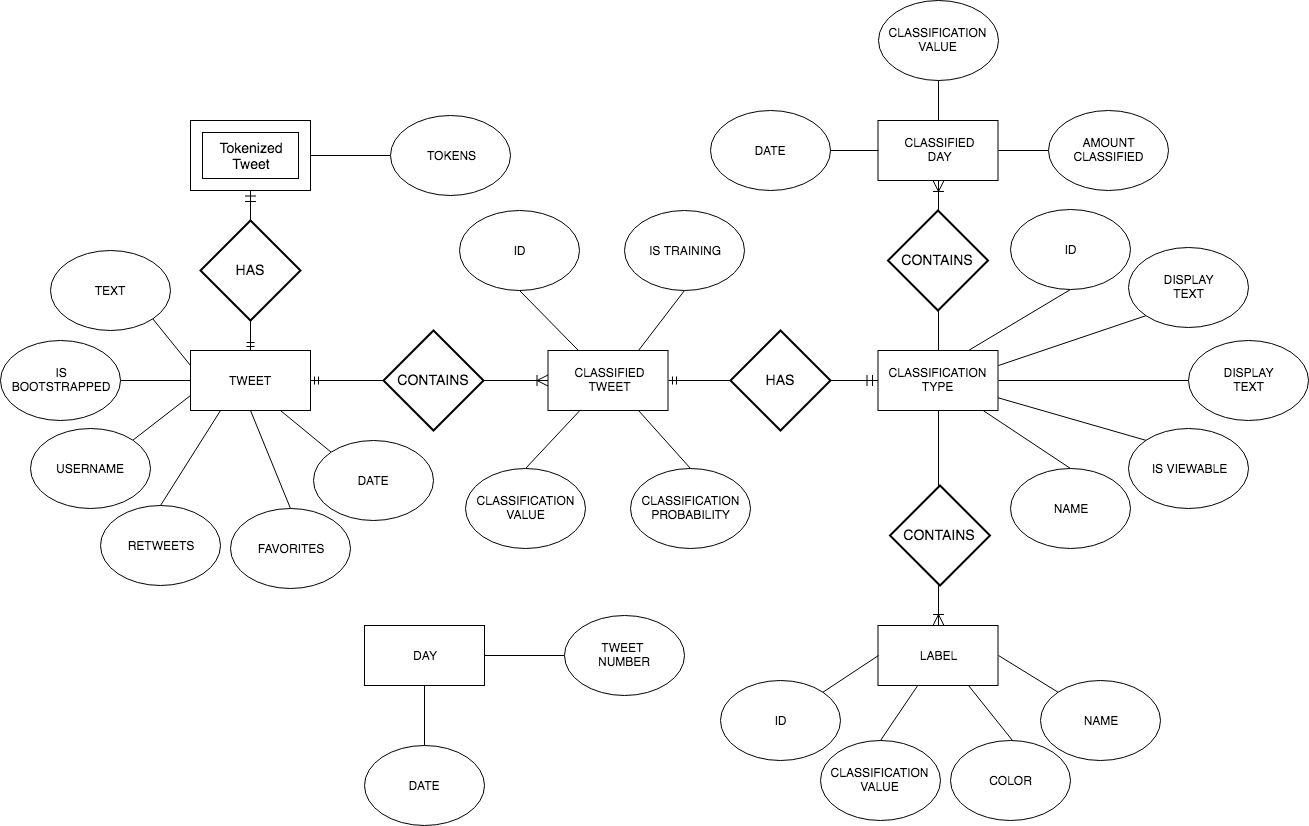
\includegraphics[width=0.7\textheight]{images/conceptual-erd.jpg}}
     {Home Page}
&
\subf{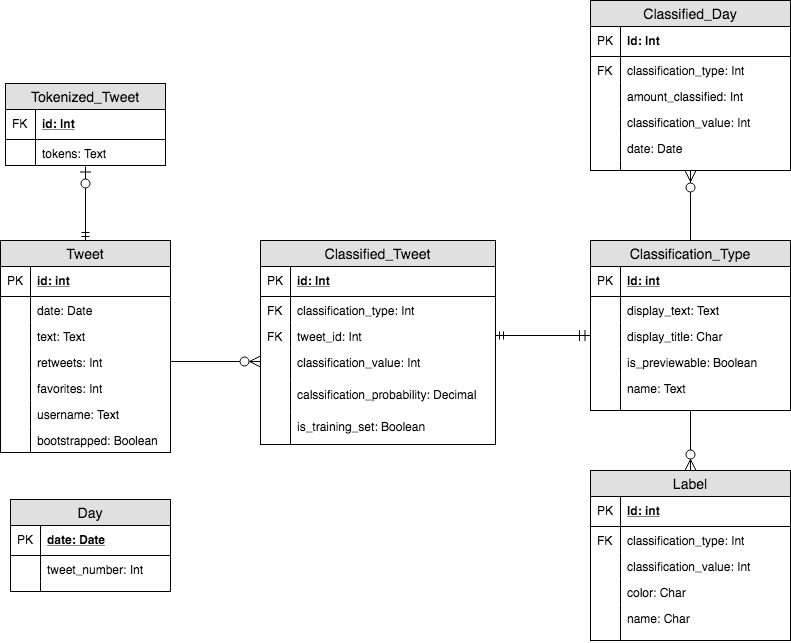
\includegraphics[width=0.7\textheight]{images/physical-erd.jpg}}
     {Analysis Page}
     \vspace{1cm}
\\
\end{tabular}
\end{figure}
\end{landscape}
\end{document} 